\subsection{Six-method cat comparison across learning rates and capacities}\label{app:flux-four}\label{app:diffusion}\label{app:extendedimage}
The complete cat study crosses six methods, four approximately matched parameter budgets, eight LRs and seeds 0, 1 and 2, giving 576 successful runs and 192 configuration means. All methods share the cat split (14 training, two validation and four test images), adapted modules, training exposure and evaluation steps. LoRA, DoRA, PiSSA and MiLoRA use ranks 4/8/16/32, OFT uses block sizes 32/64/128/256, and HRA uses 16/32/62/124 Householder vectors. PiSSA/MiLoRA ranks refer to training, with doubled ranks used to serialize their differences from the base model.

The LR grid is $\{5\times10^{-6},10^{-5},3\times10^{-5},5\times10^{-5},10^{-4},3\times10^{-4},5\times10^{-4},10^{-3}\}$. Within each method/capacity, mean validation DINO at step 700 selects one LR shared across seeds, with ties favoring smaller LR. Test and retention use step 750. \Cref{tab:flux-selected-all} gives all 24 selections and parameter counts, with sample seed SD. 

\begin{table}[!htbp]
\caption{Complete validation-selected FLUX cat results. Budgets are approximately matched, with HRA using 16/32/62/124 vectors and DoRA adding magnitude parameters. Parameters are in millions. Validation DINO at step 700 selects LR separately for each method/capacity. Step 750 supplies test DINO, general drift and general CLIP. Scores are $\times100$.}
\label{tab:flux-selected-all}
\begin{center}
\setlength{\tabcolsep}{3pt}
\begin{tabular*}{\linewidth}{@{\extracolsep{\fill}}lccccccc@{}}\toprule
Method & Capacity & Params & LR & Validation & Test DINO & Gen. drift & Gen. CLIP \\ \midrule
\textcolor{LoRAColor}{LoRA} & r4 & \result{ext_flux_flux_lora_cap4_0p0003_params} & $3\times10^{-4}$ & $\result{ext_flux_flux_lora_cap4_0p0003_validation_mean}_{\pm\result{ext_flux_flux_lora_cap4_0p0003_validation_sd}}$ & $\result{ext_flux_flux_lora_cap4_0p0003_dino_mean}_{\pm\result{ext_flux_flux_lora_cap4_0p0003_dino_sd}}$ & $\result{ext_flux_flux_lora_cap4_0p0003_drift_mean}_{\pm\result{ext_flux_flux_lora_cap4_0p0003_drift_sd}}$ & $\result{ext_flux_flux_lora_cap4_0p0003_clip_mean}_{\pm\result{ext_flux_flux_lora_cap4_0p0003_clip_sd}}$ \\
\textcolor{OFTColor}{OFT} & b32 & \result{ext_flux_flux_oft_cap32_0p0003_params} & $3\times10^{-4}$ & $\result{ext_flux_flux_oft_cap32_0p0003_validation_mean}_{\pm\result{ext_flux_flux_oft_cap32_0p0003_validation_sd}}$ & $\result{ext_flux_flux_oft_cap32_0p0003_dino_mean}_{\pm\result{ext_flux_flux_oft_cap32_0p0003_dino_sd}}$ & $\result{ext_flux_flux_oft_cap32_0p0003_drift_mean}_{\pm\result{ext_flux_flux_oft_cap32_0p0003_drift_sd}}$ & $\result{ext_flux_flux_oft_cap32_0p0003_clip_mean}_{\pm\result{ext_flux_flux_oft_cap32_0p0003_clip_sd}}$ \\
\textcolor{DoRAColor}{DoRA} & r4 & \result{ext_flux_flux_dora_cap4_0p0005_params} & $5\times10^{-4}$ & $\result{ext_flux_flux_dora_cap4_0p0005_validation_mean}_{\pm\result{ext_flux_flux_dora_cap4_0p0005_validation_sd}}$ & $\result{ext_flux_flux_dora_cap4_0p0005_dino_mean}_{\pm\result{ext_flux_flux_dora_cap4_0p0005_dino_sd}}$ & $\result{ext_flux_flux_dora_cap4_0p0005_drift_mean}_{\pm\result{ext_flux_flux_dora_cap4_0p0005_drift_sd}}$ & $\result{ext_flux_flux_dora_cap4_0p0005_clip_mean}_{\pm\result{ext_flux_flux_dora_cap4_0p0005_clip_sd}}$ \\
\textcolor{PiSSAColor}{PiSSA} & r4 & \result{ext_flux_flux_pissa_cap4_0p0001_params} & $1\times10^{-4}$ & $\result{ext_flux_flux_pissa_cap4_0p0001_validation_mean}_{\pm\result{ext_flux_flux_pissa_cap4_0p0001_validation_sd}}$ & $\result{ext_flux_flux_pissa_cap4_0p0001_dino_mean}_{\pm\result{ext_flux_flux_pissa_cap4_0p0001_dino_sd}}$ & $\result{ext_flux_flux_pissa_cap4_0p0001_drift_mean}_{\pm\result{ext_flux_flux_pissa_cap4_0p0001_drift_sd}}$ & $\result{ext_flux_flux_pissa_cap4_0p0001_clip_mean}_{\pm\result{ext_flux_flux_pissa_cap4_0p0001_clip_sd}}$ \\
\textcolor{MiLoRAColor}{MiLoRA} & r4 & \result{ext_flux_flux_milora_cap4_0p0001_params} & $1\times10^{-4}$ & $\result{ext_flux_flux_milora_cap4_0p0001_validation_mean}_{\pm\result{ext_flux_flux_milora_cap4_0p0001_validation_sd}}$ & $\result{ext_flux_flux_milora_cap4_0p0001_dino_mean}_{\pm\result{ext_flux_flux_milora_cap4_0p0001_dino_sd}}$ & $\result{ext_flux_flux_milora_cap4_0p0001_drift_mean}_{\pm\result{ext_flux_flux_milora_cap4_0p0001_drift_sd}}$ & $\result{ext_flux_flux_milora_cap4_0p0001_clip_mean}_{\pm\result{ext_flux_flux_milora_cap4_0p0001_clip_sd}}$ \\
\textcolor{HRAColor}{HRA} & h16 & \result{ext_flux_flux_hra_cap16_0p0005_params} & $5\times10^{-4}$ & $\result{ext_flux_flux_hra_cap16_0p0005_validation_mean}_{\pm\result{ext_flux_flux_hra_cap16_0p0005_validation_sd}}$ & $\result{ext_flux_flux_hra_cap16_0p0005_dino_mean}_{\pm\result{ext_flux_flux_hra_cap16_0p0005_dino_sd}}$ & $\result{ext_flux_flux_hra_cap16_0p0005_drift_mean}_{\pm\result{ext_flux_flux_hra_cap16_0p0005_drift_sd}}$ & $\result{ext_flux_flux_hra_cap16_0p0005_clip_mean}_{\pm\result{ext_flux_flux_hra_cap16_0p0005_clip_sd}}$ \\
\midrule
\textcolor{LoRAColor}{LoRA} & r8 & \result{ext_flux_flux_lora_0p0001_params} & $1\times10^{-4}$ & $\result{ext_flux_flux_lora_0p0001_validation_mean}_{\pm\result{ext_flux_flux_lora_0p0001_validation_sd}}$ & $\result{ext_flux_flux_lora_0p0001_dino_mean}_{\pm\result{ext_flux_flux_lora_0p0001_dino_sd}}$ & $\result{ext_flux_flux_lora_0p0001_drift_mean}_{\pm\result{ext_flux_flux_lora_0p0001_drift_sd}}$ & $\result{ext_flux_flux_lora_0p0001_clip_mean}_{\pm\result{ext_flux_flux_lora_0p0001_clip_sd}}$ \\
\textcolor{OFTColor}{OFT} & b64 & \result{ext_flux_flux_oft_5em05_params} & $5\times10^{-5}$ & $\result{ext_flux_flux_oft_5em05_validation_mean}_{\pm\result{ext_flux_flux_oft_5em05_validation_sd}}$ & $\result{ext_flux_flux_oft_5em05_dino_mean}_{\pm\result{ext_flux_flux_oft_5em05_dino_sd}}$ & $\result{ext_flux_flux_oft_5em05_drift_mean}_{\pm\result{ext_flux_flux_oft_5em05_drift_sd}}$ & $\result{ext_flux_flux_oft_5em05_clip_mean}_{\pm\result{ext_flux_flux_oft_5em05_clip_sd}}$ \\
\textcolor{DoRAColor}{DoRA} & r8 & \result{ext_flux_flux_dora_0p0003_params} & $3\times10^{-4}$ & $\result{ext_flux_flux_dora_0p0003_validation_mean}_{\pm\result{ext_flux_flux_dora_0p0003_validation_sd}}$ & $\result{ext_flux_flux_dora_0p0003_dino_mean}_{\pm\result{ext_flux_flux_dora_0p0003_dino_sd}}$ & $\result{ext_flux_flux_dora_0p0003_drift_mean}_{\pm\result{ext_flux_flux_dora_0p0003_drift_sd}}$ & $\result{ext_flux_flux_dora_0p0003_clip_mean}_{\pm\result{ext_flux_flux_dora_0p0003_clip_sd}}$ \\
\textcolor{PiSSAColor}{PiSSA} & r8 & \result{ext_flux_flux_pissa_5em05_params} & $5\times10^{-5}$ & $\result{ext_flux_flux_pissa_5em05_validation_mean}_{\pm\result{ext_flux_flux_pissa_5em05_validation_sd}}$ & $\result{ext_flux_flux_pissa_5em05_dino_mean}_{\pm\result{ext_flux_flux_pissa_5em05_dino_sd}}$ & $\result{ext_flux_flux_pissa_5em05_drift_mean}_{\pm\result{ext_flux_flux_pissa_5em05_drift_sd}}$ & $\result{ext_flux_flux_pissa_5em05_clip_mean}_{\pm\result{ext_flux_flux_pissa_5em05_clip_sd}}$ \\
\textcolor{MiLoRAColor}{MiLoRA} & r8 & \result{ext_flux_flux_milora_5em05_params} & $5\times10^{-5}$ & $\result{ext_flux_flux_milora_5em05_validation_mean}_{\pm\result{ext_flux_flux_milora_5em05_validation_sd}}$ & $\result{ext_flux_flux_milora_5em05_dino_mean}_{\pm\result{ext_flux_flux_milora_5em05_dino_sd}}$ & $\result{ext_flux_flux_milora_5em05_drift_mean}_{\pm\result{ext_flux_flux_milora_5em05_drift_sd}}$ & $\result{ext_flux_flux_milora_5em05_clip_mean}_{\pm\result{ext_flux_flux_milora_5em05_clip_sd}}$ \\
\textcolor{HRAColor}{HRA} & h32 & \result{ext_flux_flux_hra_0p0003_params} & $3\times10^{-4}$ & $\result{ext_flux_flux_hra_0p0003_validation_mean}_{\pm\result{ext_flux_flux_hra_0p0003_validation_sd}}$ & $\result{ext_flux_flux_hra_0p0003_dino_mean}_{\pm\result{ext_flux_flux_hra_0p0003_dino_sd}}$ & $\result{ext_flux_flux_hra_0p0003_drift_mean}_{\pm\result{ext_flux_flux_hra_0p0003_drift_sd}}$ & $\result{ext_flux_flux_hra_0p0003_clip_mean}_{\pm\result{ext_flux_flux_hra_0p0003_clip_sd}}$ \\
\midrule
\textcolor{LoRAColor}{LoRA} & r16 & \result{ext_flux_flux_lora_cap16_0p0001_params} & $1\times10^{-4}$ & $\result{ext_flux_flux_lora_cap16_0p0001_validation_mean}_{\pm\result{ext_flux_flux_lora_cap16_0p0001_validation_sd}}$ & $\result{ext_flux_flux_lora_cap16_0p0001_dino_mean}_{\pm\result{ext_flux_flux_lora_cap16_0p0001_dino_sd}}$ & $\result{ext_flux_flux_lora_cap16_0p0001_drift_mean}_{\pm\result{ext_flux_flux_lora_cap16_0p0001_drift_sd}}$ & $\result{ext_flux_flux_lora_cap16_0p0001_clip_mean}_{\pm\result{ext_flux_flux_lora_cap16_0p0001_clip_sd}}$ \\
\textcolor{OFTColor}{OFT} & b128 & \result{ext_flux_flux_oft_cap128_0p0001_params} & $1\times10^{-4}$ & $\result{ext_flux_flux_oft_cap128_0p0001_validation_mean}_{\pm\result{ext_flux_flux_oft_cap128_0p0001_validation_sd}}$ & $\result{ext_flux_flux_oft_cap128_0p0001_dino_mean}_{\pm\result{ext_flux_flux_oft_cap128_0p0001_dino_sd}}$ & $\result{ext_flux_flux_oft_cap128_0p0001_drift_mean}_{\pm\result{ext_flux_flux_oft_cap128_0p0001_drift_sd}}$ & $\result{ext_flux_flux_oft_cap128_0p0001_clip_mean}_{\pm\result{ext_flux_flux_oft_cap128_0p0001_clip_sd}}$ \\
\textcolor{DoRAColor}{DoRA} & r16 & \result{ext_flux_flux_dora_cap16_5em05_params} & $5\times10^{-5}$ & $\result{ext_flux_flux_dora_cap16_5em05_validation_mean}_{\pm\result{ext_flux_flux_dora_cap16_5em05_validation_sd}}$ & $\result{ext_flux_flux_dora_cap16_5em05_dino_mean}_{\pm\result{ext_flux_flux_dora_cap16_5em05_dino_sd}}$ & $\result{ext_flux_flux_dora_cap16_5em05_drift_mean}_{\pm\result{ext_flux_flux_dora_cap16_5em05_drift_sd}}$ & $\result{ext_flux_flux_dora_cap16_5em05_clip_mean}_{\pm\result{ext_flux_flux_dora_cap16_5em05_clip_sd}}$ \\
\textcolor{PiSSAColor}{PiSSA} & r16 & \result{ext_flux_flux_pissa_cap16_5em05_params} & $5\times10^{-5}$ & $\result{ext_flux_flux_pissa_cap16_5em05_validation_mean}_{\pm\result{ext_flux_flux_pissa_cap16_5em05_validation_sd}}$ & $\result{ext_flux_flux_pissa_cap16_5em05_dino_mean}_{\pm\result{ext_flux_flux_pissa_cap16_5em05_dino_sd}}$ & $\result{ext_flux_flux_pissa_cap16_5em05_drift_mean}_{\pm\result{ext_flux_flux_pissa_cap16_5em05_drift_sd}}$ & $\result{ext_flux_flux_pissa_cap16_5em05_clip_mean}_{\pm\result{ext_flux_flux_pissa_cap16_5em05_clip_sd}}$ \\
\textcolor{MiLoRAColor}{MiLoRA} & r16 & \result{ext_flux_flux_milora_cap16_0p0001_params} & $1\times10^{-4}$ & $\result{ext_flux_flux_milora_cap16_0p0001_validation_mean}_{\pm\result{ext_flux_flux_milora_cap16_0p0001_validation_sd}}$ & $\result{ext_flux_flux_milora_cap16_0p0001_dino_mean}_{\pm\result{ext_flux_flux_milora_cap16_0p0001_dino_sd}}$ & $\result{ext_flux_flux_milora_cap16_0p0001_drift_mean}_{\pm\result{ext_flux_flux_milora_cap16_0p0001_drift_sd}}$ & $\result{ext_flux_flux_milora_cap16_0p0001_clip_mean}_{\pm\result{ext_flux_flux_milora_cap16_0p0001_clip_sd}}$ \\
\textcolor{HRAColor}{HRA} & h62 & \result{ext_flux_flux_hra_cap62_0p0005_params} & $5\times10^{-4}$ & $\result{ext_flux_flux_hra_cap62_0p0005_validation_mean}_{\pm\result{ext_flux_flux_hra_cap62_0p0005_validation_sd}}$ & $\result{ext_flux_flux_hra_cap62_0p0005_dino_mean}_{\pm\result{ext_flux_flux_hra_cap62_0p0005_dino_sd}}$ & $\result{ext_flux_flux_hra_cap62_0p0005_drift_mean}_{\pm\result{ext_flux_flux_hra_cap62_0p0005_drift_sd}}$ & $\result{ext_flux_flux_hra_cap62_0p0005_clip_mean}_{\pm\result{ext_flux_flux_hra_cap62_0p0005_clip_sd}}$ \\
\midrule
\textcolor{LoRAColor}{LoRA} & r32 & \result{ext_flux_flux_lora_cap32_5em05_params} & $5\times10^{-5}$ & $\result{ext_flux_flux_lora_cap32_5em05_validation_mean}_{\pm\result{ext_flux_flux_lora_cap32_5em05_validation_sd}}$ & $\result{ext_flux_flux_lora_cap32_5em05_dino_mean}_{\pm\result{ext_flux_flux_lora_cap32_5em05_dino_sd}}$ & $\result{ext_flux_flux_lora_cap32_5em05_drift_mean}_{\pm\result{ext_flux_flux_lora_cap32_5em05_drift_sd}}$ & $\result{ext_flux_flux_lora_cap32_5em05_clip_mean}_{\pm\result{ext_flux_flux_lora_cap32_5em05_clip_sd}}$ \\
\textcolor{OFTColor}{OFT} & b256 & \result{ext_flux_flux_oft_cap256_0p0001_params} & $1\times10^{-4}$ & $\result{ext_flux_flux_oft_cap256_0p0001_validation_mean}_{\pm\result{ext_flux_flux_oft_cap256_0p0001_validation_sd}}$ & $\result{ext_flux_flux_oft_cap256_0p0001_dino_mean}_{\pm\result{ext_flux_flux_oft_cap256_0p0001_dino_sd}}$ & $\result{ext_flux_flux_oft_cap256_0p0001_drift_mean}_{\pm\result{ext_flux_flux_oft_cap256_0p0001_drift_sd}}$ & $\result{ext_flux_flux_oft_cap256_0p0001_clip_mean}_{\pm\result{ext_flux_flux_oft_cap256_0p0001_clip_sd}}$ \\
\textcolor{DoRAColor}{DoRA} & r32 & \result{ext_flux_flux_dora_cap32_0p0001_params} & $1\times10^{-4}$ & $\result{ext_flux_flux_dora_cap32_0p0001_validation_mean}_{\pm\result{ext_flux_flux_dora_cap32_0p0001_validation_sd}}$ & $\result{ext_flux_flux_dora_cap32_0p0001_dino_mean}_{\pm\result{ext_flux_flux_dora_cap32_0p0001_dino_sd}}$ & $\result{ext_flux_flux_dora_cap32_0p0001_drift_mean}_{\pm\result{ext_flux_flux_dora_cap32_0p0001_drift_sd}}$ & $\result{ext_flux_flux_dora_cap32_0p0001_clip_mean}_{\pm\result{ext_flux_flux_dora_cap32_0p0001_clip_sd}}$ \\
\textcolor{PiSSAColor}{PiSSA} & r32 & \result{ext_flux_flux_pissa_cap32_5em05_params} & $5\times10^{-5}$ & $\result{ext_flux_flux_pissa_cap32_5em05_validation_mean}_{\pm\result{ext_flux_flux_pissa_cap32_5em05_validation_sd}}$ & $\result{ext_flux_flux_pissa_cap32_5em05_dino_mean}_{\pm\result{ext_flux_flux_pissa_cap32_5em05_dino_sd}}$ & $\result{ext_flux_flux_pissa_cap32_5em05_drift_mean}_{\pm\result{ext_flux_flux_pissa_cap32_5em05_drift_sd}}$ & $\result{ext_flux_flux_pissa_cap32_5em05_clip_mean}_{\pm\result{ext_flux_flux_pissa_cap32_5em05_clip_sd}}$ \\
\textcolor{MiLoRAColor}{MiLoRA} & r32 & \result{ext_flux_flux_milora_cap32_0p0001_params} & $1\times10^{-4}$ & $\result{ext_flux_flux_milora_cap32_0p0001_validation_mean}_{\pm\result{ext_flux_flux_milora_cap32_0p0001_validation_sd}}$ & $\result{ext_flux_flux_milora_cap32_0p0001_dino_mean}_{\pm\result{ext_flux_flux_milora_cap32_0p0001_dino_sd}}$ & $\result{ext_flux_flux_milora_cap32_0p0001_drift_mean}_{\pm\result{ext_flux_flux_milora_cap32_0p0001_drift_sd}}$ & $\result{ext_flux_flux_milora_cap32_0p0001_clip_mean}_{\pm\result{ext_flux_flux_milora_cap32_0p0001_clip_sd}}$ \\
\textcolor{HRAColor}{HRA} & h124 & \result{ext_flux_flux_hra_cap124_0p0003_params} & $3\times10^{-4}$ & $\result{ext_flux_flux_hra_cap124_0p0003_validation_mean}_{\pm\result{ext_flux_flux_hra_cap124_0p0003_validation_sd}}$ & $\result{ext_flux_flux_hra_cap124_0p0003_dino_mean}_{\pm\result{ext_flux_flux_hra_cap124_0p0003_dino_sd}}$ & $\result{ext_flux_flux_hra_cap124_0p0003_drift_mean}_{\pm\result{ext_flux_flux_hra_cap124_0p0003_drift_sd}}$ & $\result{ext_flux_flux_hra_cap124_0p0003_clip_mean}_{\pm\result{ext_flux_flux_hra_cap124_0p0003_clip_sd}}$ \\
\bottomrule\end{tabular*}

\end{center}
\end{table}

\FloatBarrier

\paragraph{Low selected drift and capacity-dependent fidelity.}
LoRA has the lowest selected mean general drift at \result{cross_cat_lora_lowest} of \result{cross_cat_selected_settings} budgets and ranks among the lowest two at all \result{cross_cat_lora_lowest_two}. PiSSA has greater drift than LoRA in all \result{cross_cat_pissa_above_lora_seeds} paired seeds. PiSSA has the highest selected drift at the small budget, OFT at the smallest and largest budgets, and HRA at the medium budget. DoRA exceeds LoRA's mean test DINO at every selected budget and leads at the smallest and largest. MiLoRA has lower mean test DINO than LoRA at all four budgets, with a mean CLIP advantage only at the small budget. These results support LoRA's recurring retention advantage and DoRA's higher mean task scores, alongside setting-dependent outcomes for the other methods.

\begin{figure}[!htbp]\centering
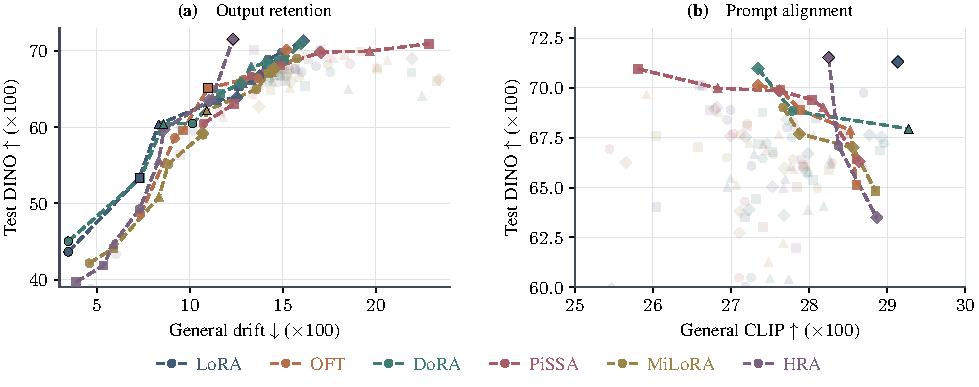
\includegraphics[width=\linewidth]{figures/flux_four_pareto.pdf}
\caption{Six-method FLUX cat test trade-offs, focused on the frontier regions. Shapes denote increasing capacity. Dashed lines and solid points mark within-method frontiers, and black borders mark the pooled frontier. Dominated points are faint. Frontiers use all 192 configurations before axis clipping, with separate y ranges for each panel. Test DINO describes final-step outcomes, while validation DINO selects LR.}
\label{fig:flux-four-pareto}
\end{figure}
\FloatBarrier

\paragraph{Retention metrics.}
General drift and CLIP use five unrelated prompts, while class drift uses five cat prompts. All six methods have these measurements. Drift measures preservation of generated outputs, and CLIP measures prompt alignment. Appendix~\ref{app:flux22} examines the role of spectral components through six-method interventions at the largest budget.
